\documentclass{article}

\usepackage{listings}
\usepackage{graphicx}
\usepackage{color} %red, green, blue, yellow, cyan, magenta, black, white
\usepackage{amsfonts}
\usepackage{mathtools}

%\newcommand\mat[1]{\mathcal{\underline{#1}}}

\definecolor{mygreen}{RGB}{28,172,0} % color values Red, Green, Blue
\definecolor{mylilas}{RGB}{170,55,241}
%% Preamble done!
%% Begin document
\begin{document}
\lstset{language=Matlab,%
    %basicstyle=\color{red},
    breaklines=true,%
    morekeywords={matlab2tikz},
    keywordstyle=\color{blue},%
    morekeywords=[2]{1}, keywordstyle=[2]{\color{black}},
    identifierstyle=\color{black},%
    stringstyle=\color{mylilas},
    commentstyle=\color{mygreen},%
    showstringspaces=false,%without this there will be a symbol in the places where there is a space
    numbers=left,%
    numberstyle={\tiny \color{black}},% size of the numbers
    numbersep=12pt, % this defines how far the numbers are from the text
    emph=[1]{for,end,break},emphstyle=[1]\color{red}, %some words to emphasise
    %emph=[2]{word1,word2}, emphstyle=[2]{style},    
}
\label{Cover}
	\begin{center}
	\large{ECE-5554 Computer Vision: Problem Set 1}
	\vfill
	Murat Ambarkutuk \\ murata@vt.edu
	\vfill
	Mechanical Engineering Department,\\ Virginia Polytechnic Institute and State University
	\vfill
	\today
	\end{center}
\pagebreak 
\large{Answer Sheet}
\label{Short Answer Problems}
\section{Short Answer Problems}
\begin{enumerate}
	% 1- Give an example of how one can exploit the associative property of
	% convolution to more efficiently filter an image.
	\item The computational complexity of convolution operation for any arbitrary
	kernel $\mat{F_0}_{[m\times n]}$ and image $\mat{I_0}_{[M\times N]}$:
	$$\matcal{O}(MNmn)$$
	Hence, applying a handful of filters will multiply
	the computational cost of filtering process.\\
	Say, $\mat{F_0}_{[m\times n]} \ast \{\mat{F_1}_{[m\times n]} \ast
	\mat{I_0}_{[M\times N]}\}$ will be computed with the complexity of $$2 \times
	\matcal{O}(MNmn)$$
	On the other hand, convolving the filters first, then applying the
	acquired filter to image will cost: $$\matcal{O}(mnmn) + \matcal{O}(MNmn)$$
	Furthermore, considering that in any filtering process the size of filter
	kernell will be smaller than the image size, $$\matcal{O}(mnmn) + \matcal{O}(MNmn) < 2 \times \matcal{O}(MNmn)$$.
	% 2- This is the input image: [0 0 1 1 0 0 1 1]. What is the result of dilation
	% with a structuring element [1 1 1]?
	\item 
	$$\vec{I} = \begin{bmatrix} 0 & 0 & 1 & 1 & 0 & 0 & 1 & 1\end{bmatrix}
	, \vec{f}= \begin{bmatrix} 1 & 1 & 1\end{bmatrix}$$
	\begin{equation} 
	\begin{split}
	\vec{H} & = \vec{I} \ast \vec{f} \\
	& = \begin{bmatrix} 0 & 1 & 2 & 2 & 1 & 1 & 2 & 2 \end{bmatrix}
	\end{split}
	\end{equation}
	% 3- The filter f’ = [0 -1/2 0 1/2 0] gives an estimate of the first derivative
	% of the image in the x direction.
	% What is the corresponding second derivative filter f". (Hint: Assymetric
	% filters must be flipped prior to convolution.)
	\item $ \vec{f''} = \begin{bmatrix} 0 & 0 & 1/4 & 0 & -1/2 & 0 & 1/4 & 0 & 0
	\end{bmatrix}$
	% 4- Name two specific ways in which one could reduce the amount of fine, detailed edges that are detected
	% with the Canny edge detector.
	\item
	\begin{enumerate}
		\item Low threshold:
		\item High threshold:	
	\end{enumerate}
	% 5- Describe a possible flaw in the use of additive Gaussian noise to
	% represent image noise.
	\item In real world applications noise occuring in the image may vary
	depending on many variables, namely, the lightning conditions of the
	environment in which the camera set up or the type of sensor that are being
	used. For that reason, modeling the noise with Gaussian noise may not describe
	the real world for each case of application. 
	% 6- Design a method that takes video data from a camera perched above a conveyor belt at an automotive
	% equipment manufacturer, and reports any flaws in the assembly of a part. Your
	% response should be a list of concise, specific steps, and should incorporate
	% several techniques covered in class thus far.
	% Specify any important assumptions your method makes. 
	\item A tentative flow of solution can be used for many generic vision
	problems:
	\begin{enumerate}
		\item Problem Definition
		\begin{enumerate}
			\item Problem definition
			\item Equipment decision based on the problem
			\item 
		\end{enumerate}
		\item Pre-processing (Preparation)
		\begin{enumerate}
			\item Data Reduction (Downsampling, color space change (RGB, $\to$,
			Grayscale, defining region of interest \ldots)
			\item Noise reduction
			\item Feature enhancing 
		\end{enumerate}
		\item Processing (Analysis)
		\begin{enumerate}
	    	\item Keypoint detection (feature detection)
	    	\item Keypoint clustering (to detect whether or not the keypoint is really
	    	a feature)
	    	\item Analysis of features
	    	\item Reporting
		\end{enumerate}
%		\item Post-processing (Interpretation)
%		\begin{enumerate}
%	    	\item 
%		\end{enumerate}
	\end{enumerate}
\end{enumerate}
\pagebreak

\label{Programming Problem (Seam Carving)}
\section{Programming Problem (Seam Carving)}
\begin{enumerate}
	\item 
	% Write a script called SeamCarvingReduceWidth.m(py) which does the following by using
	% the functions defined above:
	% (a) Loads a color input image called inputSeamCarvingPrague.jpg. Download the
	% image from here (http://filebox.ece.vt.edu/~F15ECE5554ECE4984/resources/images/inputSeamCarvingPrague.
	% jpg)
	% 2(b) Reduces the width of the image by 100 pixels using the above functions.
	% (c) Saves the resulting image as outputReduceWidthPrague.png. Submit it.
	% Display this output in your answer sheet. Submit the script.
	% (d) Repeat the steps for an input image called inputSeamCarvingMall.jpg.
	% Download the image from here
	
	% (http://filebox.ece.vt.edu/~F15ECE5554ECE4984/resources/images/inputSeamCarvingMall.
	% jpg). Save the output as outputReduceWidthMall.png. Display the output in
	% your answer sheet.
	\begin{enumerate}
		% subplot would be good 
		\item Prague (Width Resizing) \\
		%% add title and size \ldots
		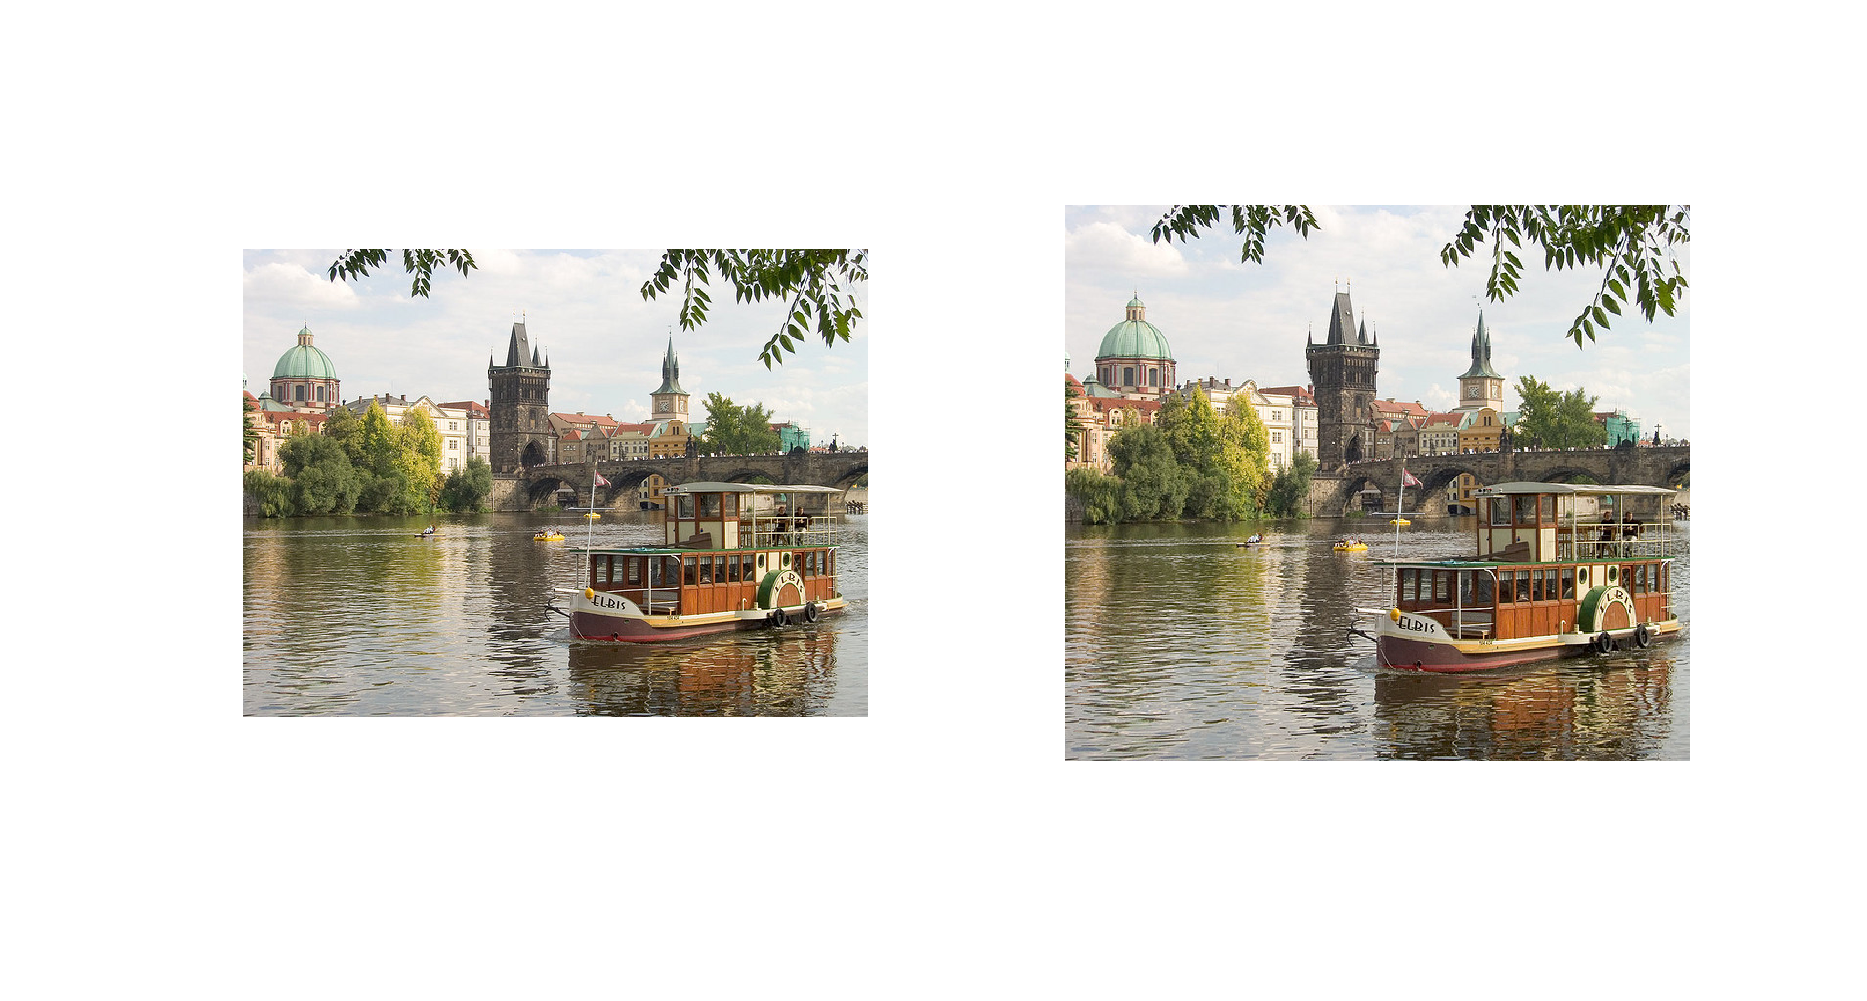
\includegraphics[width=\linewidth]{../matlab/outputPrague.png}
		\item Mall (Width Resizing)\\
		%% add titlle and size \ldots, add subplots, change picture with the correct
		% one
		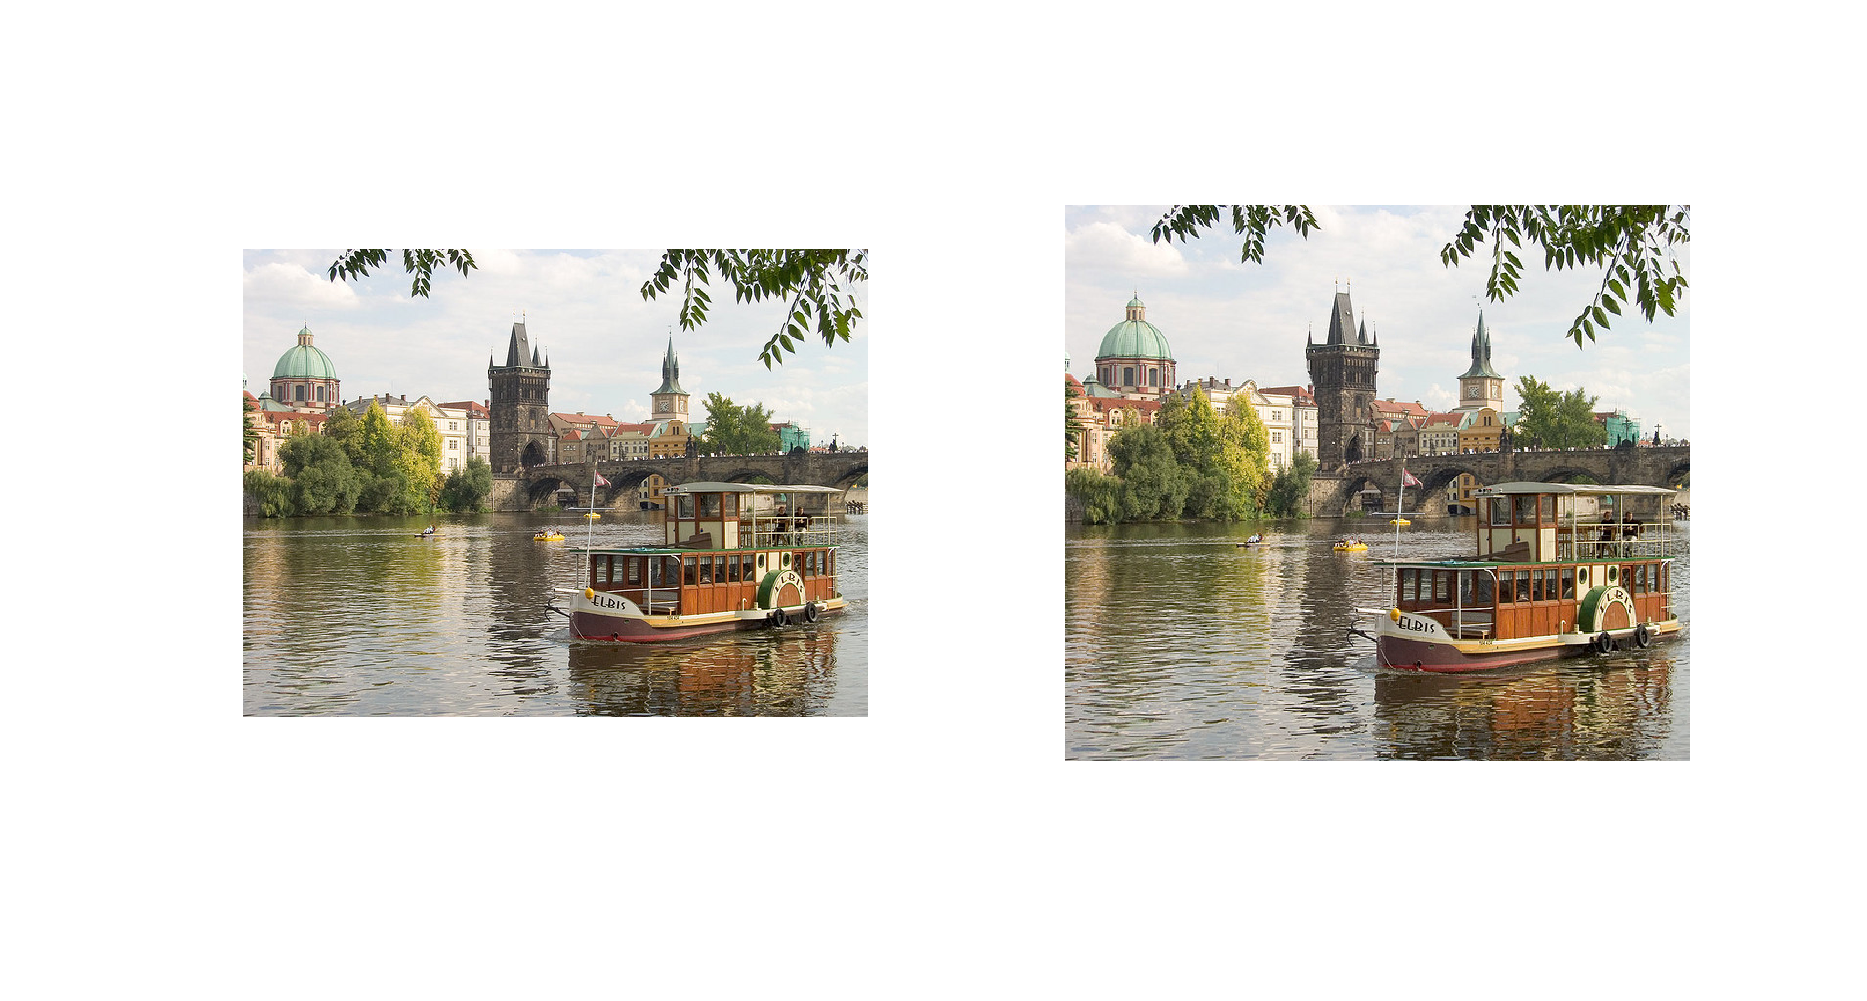
\includegraphics[width=\linewidth]{../matlab/outputPrague.png}
	\end{enumerate}
	\item
	% Repeat the above steps for both the input images, but reduce the height by 100 pixels.
	% Call the script SeamCarvingReduceHeight.m(py), and save the output images as
	% outputReduceHeightPrague.png and outputReduceHeightMall.png respectively.
	% Display both the outputs in your answer sheet. Submit the script which loads the image inputSeamCarvingPrague.jpg
	\begin{enumerate}
		% subplot would be good 
		\item Prague (Height Resizing)\\
		%% add title and size \ldots
		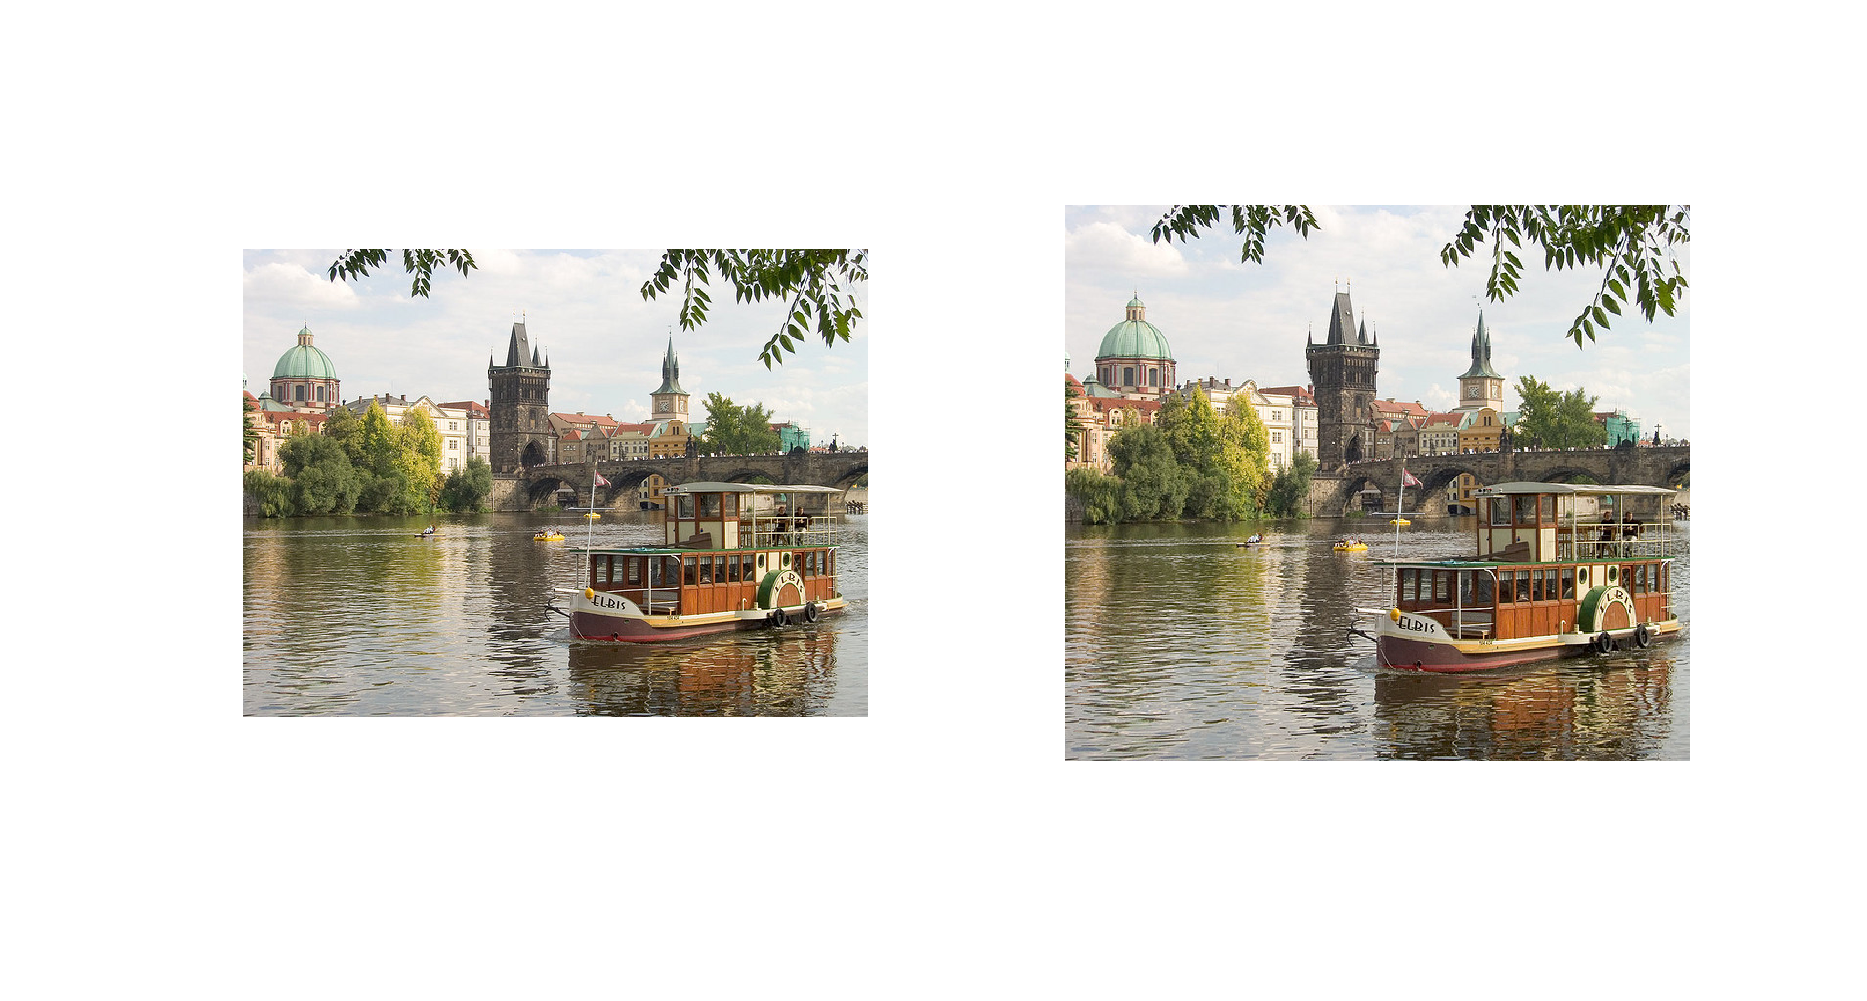
\includegraphics[width=\linewidth]{../matlab/outputPrague.png}
		\item Mall (Height Resizing)\\
		%% add titlle and size \ldots, add subplots, change picture with the correct
		% one
		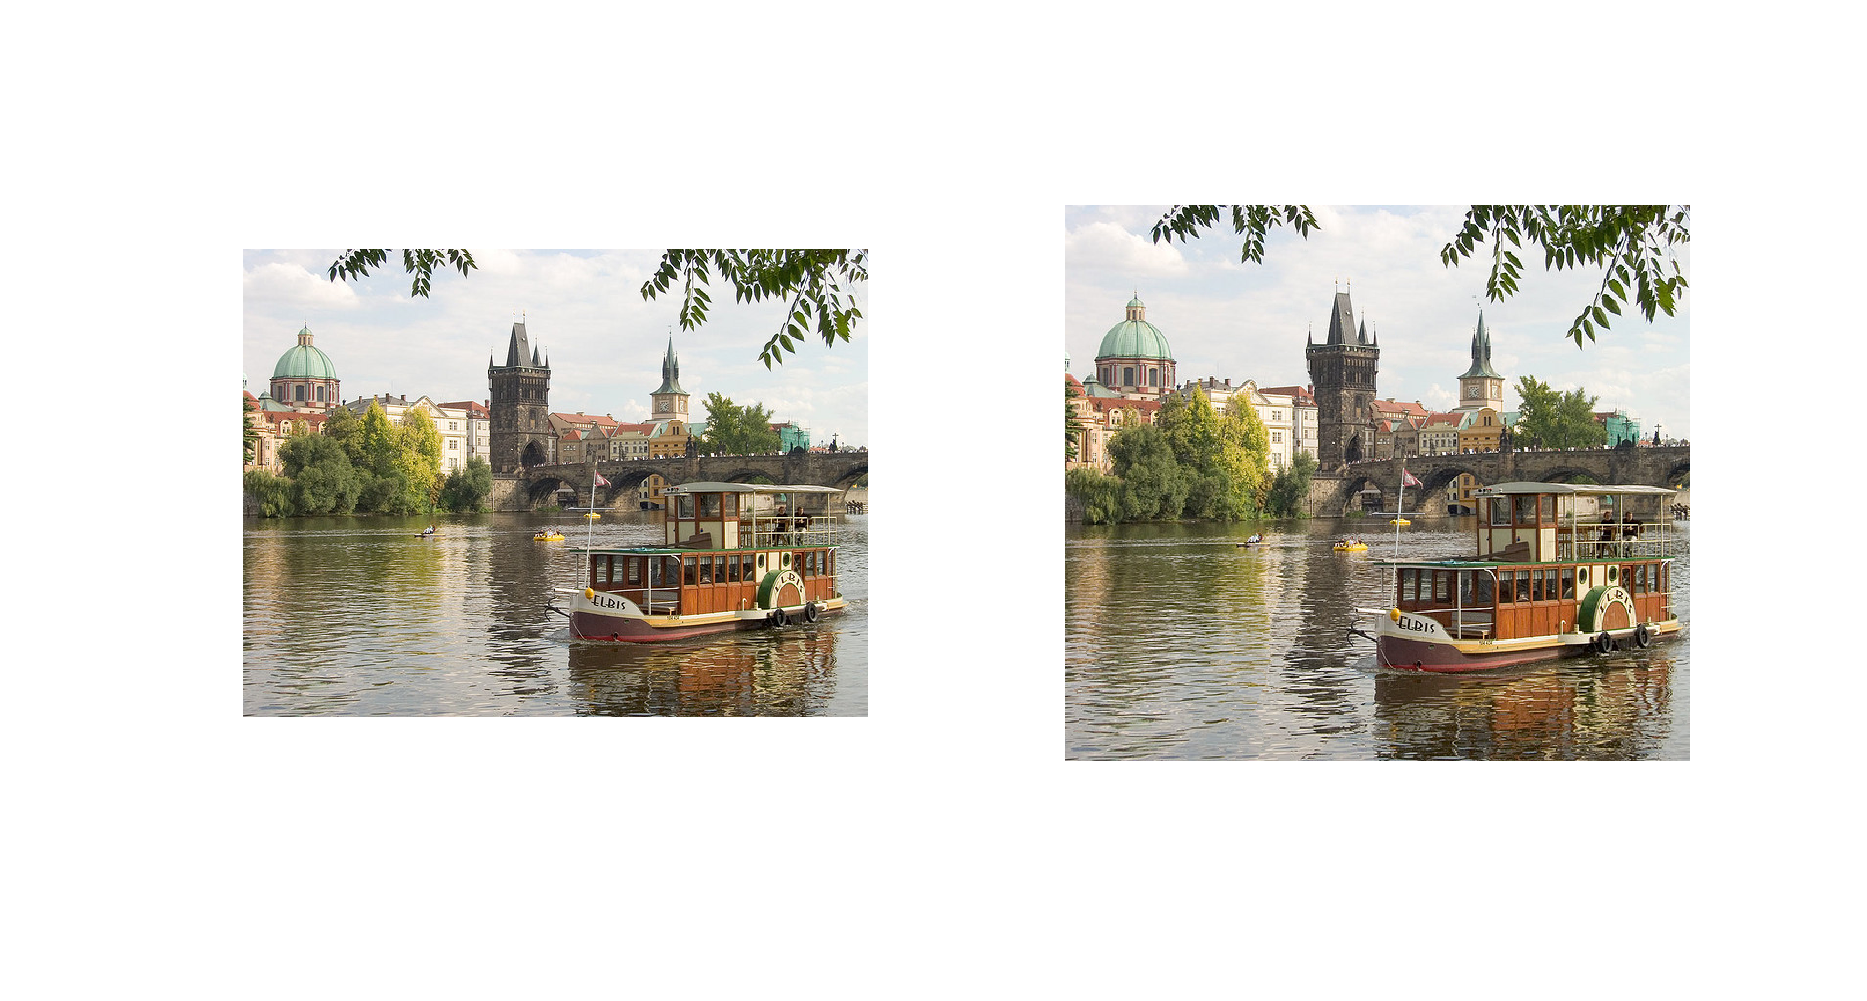
\includegraphics[width=\linewidth]{../matlab/outputPrague.png}
	\end{enumerate}
	\item
	% 3- Display in your answer sheet: (a) the energy function output for the
	% provided image inputSeamCarvingPrague.jpg, and (b) the two corresponding cumulative minimum
	% energy maps for the seams in each direction (use the Matlab’s imagesc or Python’s matplotlib.pyplot.imshow).
	% Explain why these outputs look the way they do given the original image’s
	% content.
	\begin{enumerate}
		\item Energy function output (Prague)
		\item The two corresponding cumulative energy maps for each direction \\
		Explanation for differences according to the context:
	\end{enumerate}
	\item 
	% 4- For the same image inputSeamCarvingPrague.jpg, display the original image
	% together with (a) the first selected horizontal seam and (b) the first selected
	% vertical seam in your answer sheet. Explain why these are the optimal seams for this image.
	\item
	% 5- Make some change to the way the energy function is computed (i.e., filter
	% used, its param- eters, or incorporating some other prior knowledge). Display the result and
	% explain the impact on the results for some example in your answer sheet. You need not submit this code.
	\item 
	% 6- Now, for the real results! Use your system with different kinds of images
	% and seam combi- nations, and see what kind of interesting results it can produce. The goal is
	% to form some perceptually pleasing outputs where the resizing better preserves content than a blind resizing would, as well as
	% some examples where the output looks unrealistic or has artifacts.
	% Include results for at least three images of your own choosing. Include an
	% example or two of a "bad" outcome. Be creative in the images you choose, and in the amount of combined vertical and horizontal
	% carvings you apply. Try to predict types of images where you might see
	% something interesting happen.
	% It’s ok to fiddle with the parameters (seam sequence, number of seams, etc) to
	% look for interesting and explainable outcomes.
	% For each result, include the following things, clearly labeled:
	% (a) the original input image.
	% (b) your system’s resized image,
	% (c) the result one would get if instead a simple resampling were used (via
	% Matlab’s imresize or Python’s scipy.misc.imresize)
	% (d) the input and output image dimensions,
	% (e) the sequence of removals that were used
	% (f) a qualitative explanation of what we’re seeing in the output.
\end{enumerate}
\pagebreak

\label{Extra Credit}
\section{Extra Credit}
\begin{enumerate}
	\item
	% \setcounter{enumi}{4}
	\item 
\end{enumerate}
\end{document}
